\section{Dynamic-MSV-Bench and Methodology}
\label{sec:benchmark}

We propose the \textbf{Dynamic-MSV-Bench}, which categorizes multi-shot prompts into two extreme stress-test scenarios to expose the "Double-Kill" dilemma of current models.

\begin{figure*}[ht]
    \centering
    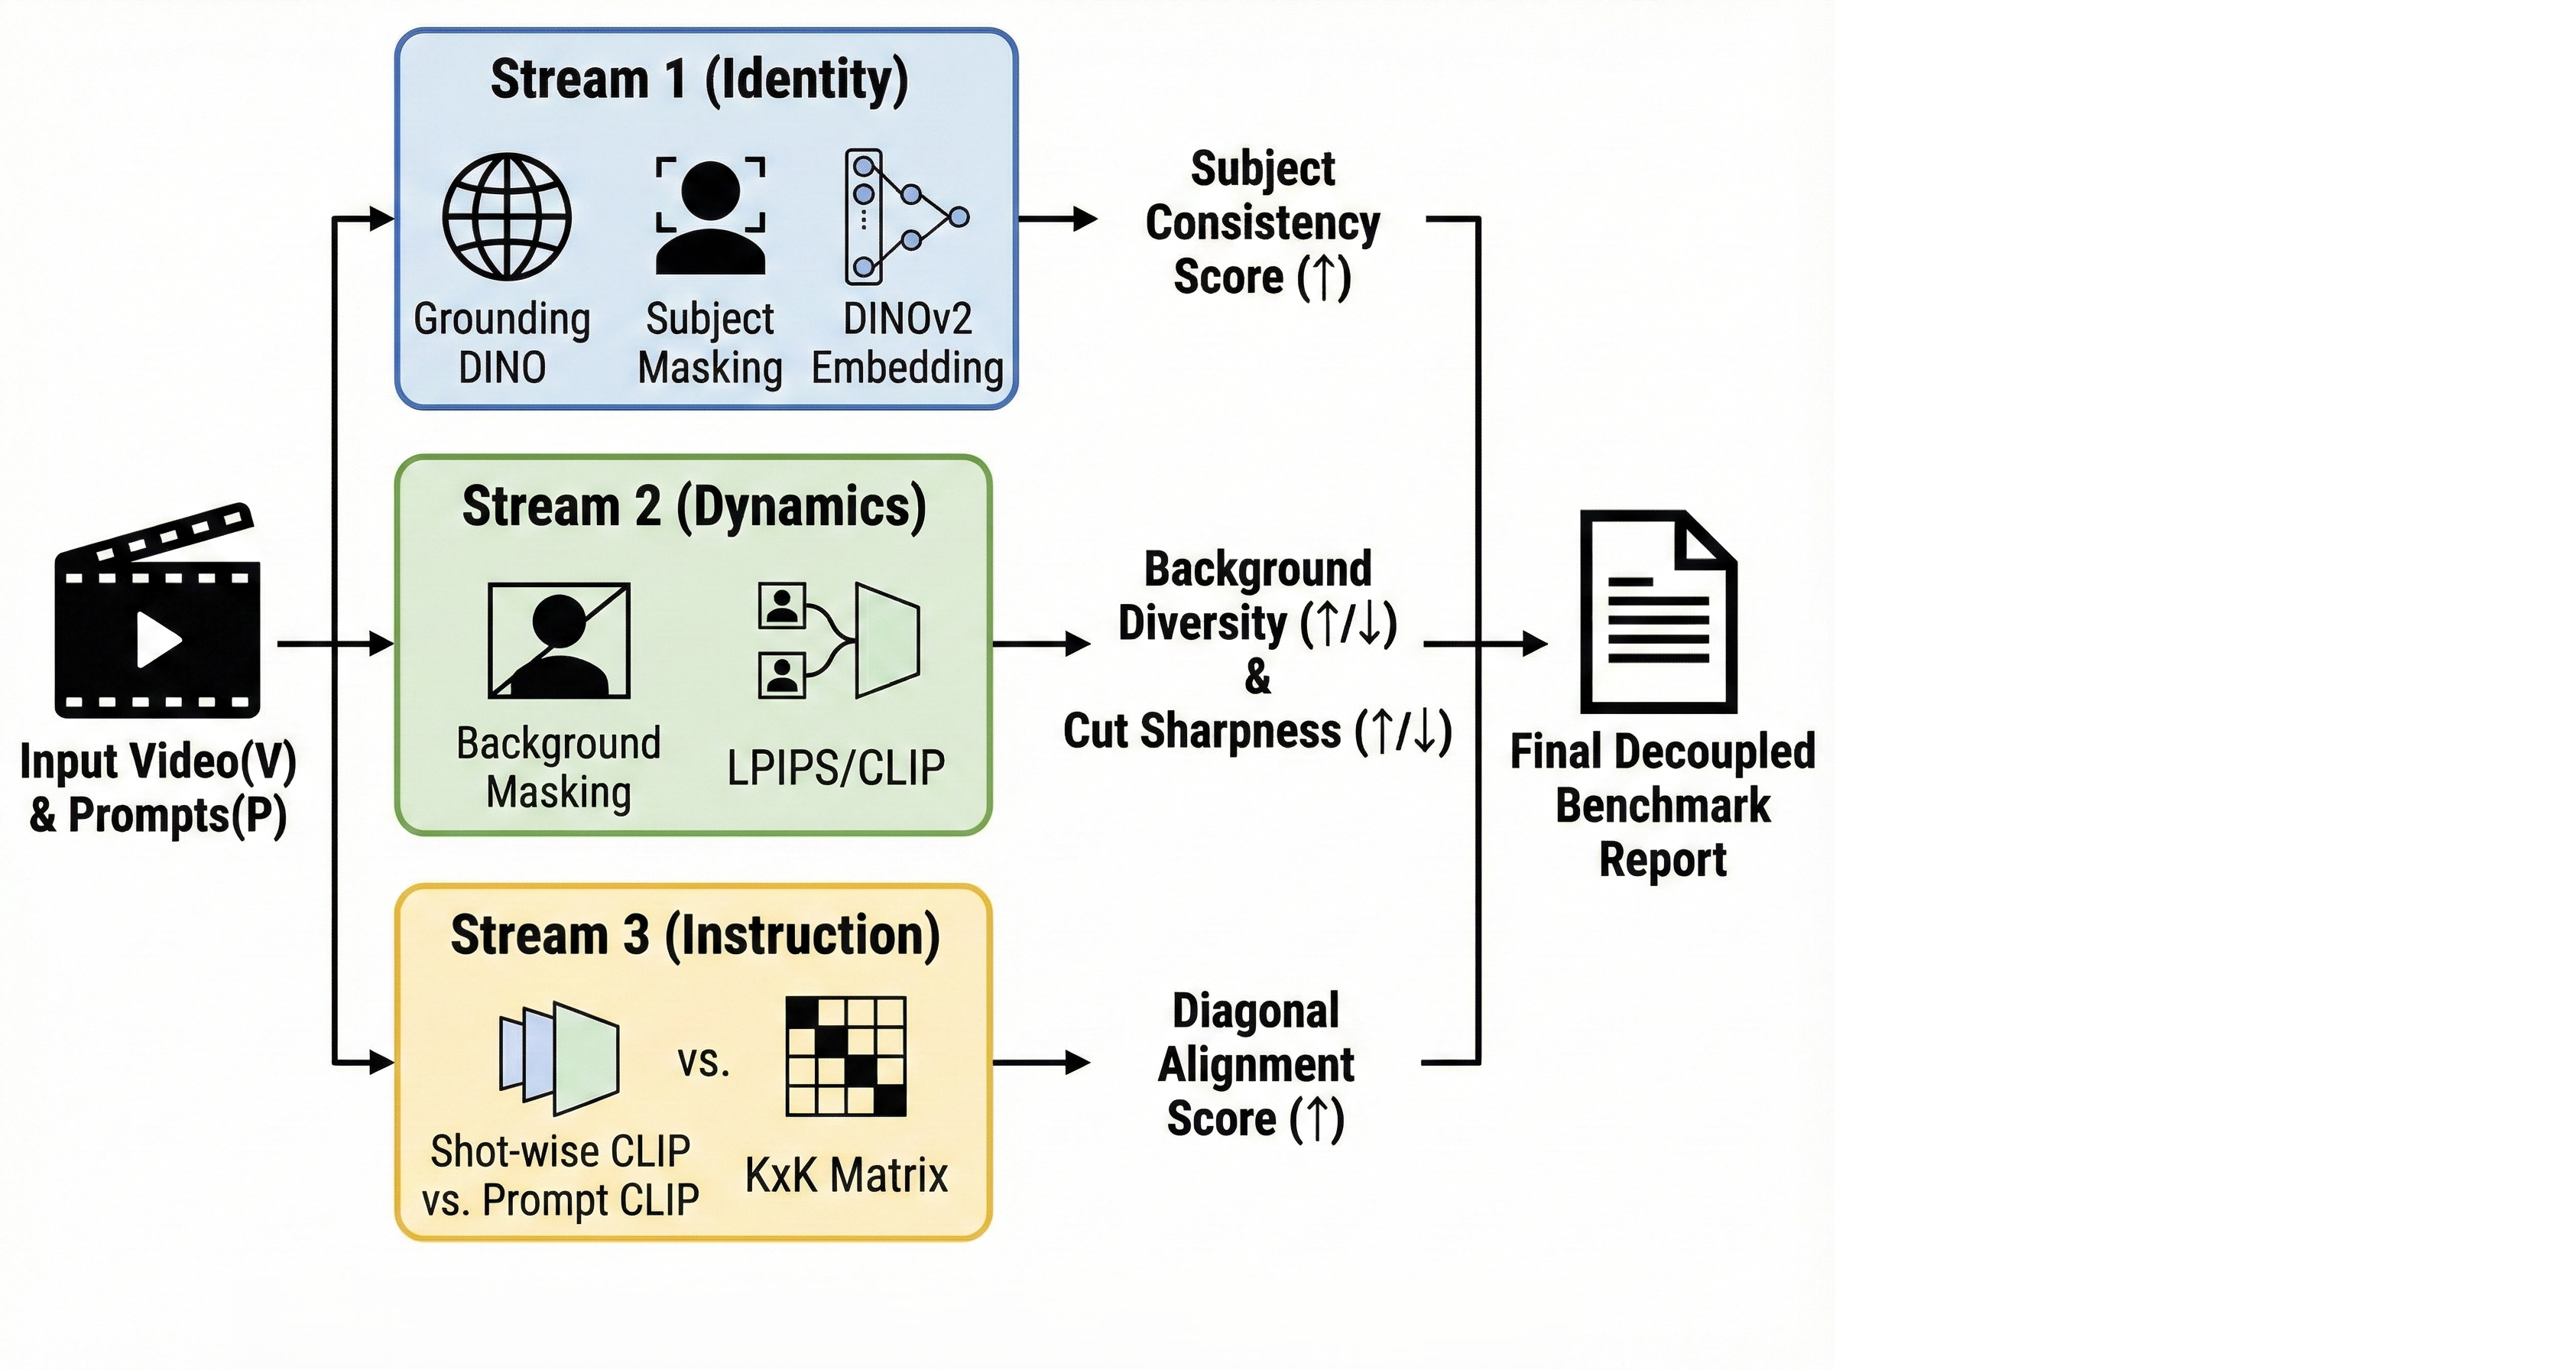
\includegraphics[width=\textwidth]{figures/fig2.png}
    \caption{Overview of our Decoupled 4D Evaluation Framework. Unlike holistic metrics like FVD, we process the input video through three independent streams to measure Subject Identity, Background Dynamics/Continuity, and Instruction Following (Diagonal Alignment) separately.}
    \label{fig:framework}
\end{figure*}

\begin{figure*}[ht]
    \centering
    \includegraphics[width=\textwidth]{figures/fig_AB.jpg}
    \caption{Conceptual comparison of our two evaluation tracks. (Left) \textbf{Track S: Semantic Leap} tests narrative diversity, requiring radical environment changes while preserving the subject. This track demands high Background Diversity and sharp cinematic cuts. (Right) \textbf{Track M: Motion Continuity} evaluates spatial integrity, where the background must remain consistent while the camera executes specific motions (Panning, Zooming, Tracking). Set M rewards low diversity and smooth spatial continuity.}
    \label{fig:sets_comparison}
\end{figure*}

\subsection{Track S: Semantic Leap (Narrative Diversity)}
Track S evaluates the model's ability to maintain a consistent subject while drastically shifting the semantic environment. 
\textbf{Golden Rule for Track S:} HIGH Background Diversity ($\uparrow$), HIGH Cut Sharpness ($\uparrow$), and HIGH Subject Consistency ($\uparrow$).

\subsection{Track M: Motion Continuity (Spatial Integrity)}
Track M tests physical instructions while keeping the background stable.
\textbf{Golden Rule for Track M:} LOW Background Diversity ($\downarrow$), LOW Cut Sharpness ($\downarrow$), and HIGH Subject Consistency ($\uparrow$).

\subsection{The 4D Decoupled Metrics}
Our framework utilizes four indices:
\begin{enumerate}
    \item \textbf{Subject Consistency ($\mathcal{C}_{subj}$):} DINOv2~\cite{oquab2023dinov2} similarity of masked subjects across shots.
    \item \textbf{Background Diversity ($\mathcal{D}_{bg}$):} Variance of CLIP/DINO embeddings in the environment region.
    \item \textbf{Cut-Transition Sharpness ($\mathcal{S}_{cut}$):} Normalized LPIPS~\cite{zhang2018perceptual} distance peaks at shot boundaries.
    \item \textbf{Diagonal Semantic Alignment (DSA):}
    Our core novelty, DSA, uses column-wise softmax probabilities:
    $$P_{i,j} = \frac{\exp(\tau \cdot M_{i,j})}{\sum_{k=1}^{K} \exp(\tau \cdot M_{k,j})}$$
    $$DSA = \frac{\left( \frac{1}{K} \sum_{i=1}^{K} P_{i,i} \right) - \frac{1}{K}}{1 - \frac{1}{K}}$$
    This formulation ensures that a static video yields a DSA of exactly 0.0.
\end{enumerate}
